\documentclass[12pt,letterpaper]{article}
\usepackage{graphicx,float}
\usepackage{hyperref}
\usepackage{amsmath,amsfonts,amssymb}

\setlength{\textwidth}{6.5in}
\setlength{\oddsidemargin}{0in}
\setlength{\textheight}{9in}
\setlength{\topmargin}{-.25in}
%DEFINE THEREFORE FUNCTION
\def\therefore{\boldsymbol{\text{ }
\leavevmode
\lower0.4ex\hbox{$\cdot$}
\kern-.5em\raise0.7ex\hbox{$\cdot$}
\kern-0.55em\lower0.4ex\hbox{$\cdot$}
\thinspace\text{ }}}

\title{Draft Report}
\author{Warvin Hassan}

\begin{document}
\maketitle
\pagebreak
\tableofcontents
\pagebreak

% PART 1
\part{Results}

% SECTION 1
\section{Paths}  \label{P}

We found that for paths the total graph value was rather trivial since there was only one spanning tree for any given path and so the product of the path is the total graph value.

% SUBSECTION 1.1
\subsection{Code}

% FIGURE 1
	\begin{figure}[hbt!]  
		\begin{center}
		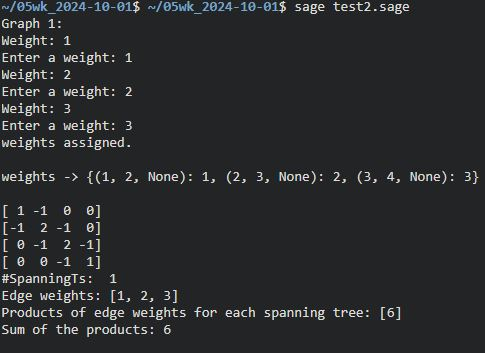
\includegraphics[width=4in]{f1.1.jpg}
		\end{center}
		\caption{\label{OrBx} Simple Path and its results using SageMath}
	\end{figure}
	

  
% SUBSECTION 1.2
\subsection{Proof}
The following proof will show that it does not matter how one assigns weights to paths by proving that the total value of the respective graph remains the same.\\

\textbf{Paths:}
Let $n\in\mathbb{Z}^{+}$, then a path $P_{n}$ on $n$ vertices has $n-1$ edges and is already a tree. It then follows, it has only one spanning tree, which is the path itself. Since the graph is trivially a tree the only spanning tree is the path itself, with the total graph value being the product of the weights of all the edges in the path $$TGV=w_{1}\cdot w_{2}\cdot\ldots\cdot w_{n-1}$$
$\therefore$ $TGV$ is an integer by the commutative laws of integer multiplication and remains the same. $\blacksquare$\\

% SECTION 2
\section{Cycles} \label{C}
Cycles were also pretty trivial as we found that regardless of the way we distributed the weights on the edges we got the same total graph value and this was due to the symmetery of cyclic graphs. We noticed that the number of spanning trees of a cycle was also the same number of vertices/edges of that same cycle.

% SUBSECTION 2.1
\subsection{Code}
 
% FIGURE 2
	\begin{figure}[h!]
  \begin{center}
    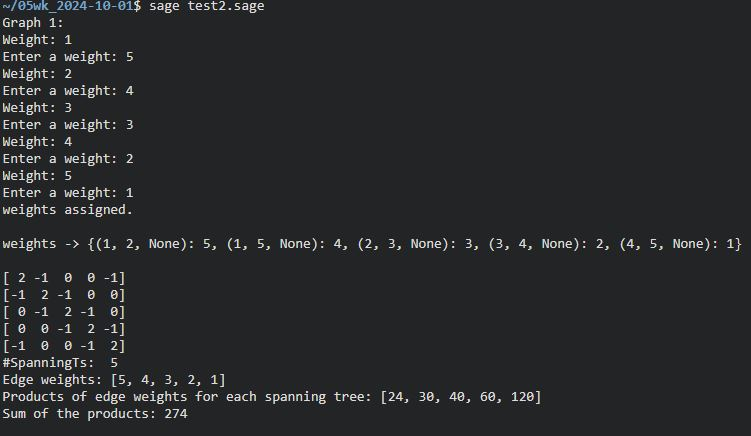
\includegraphics[width=4.2in]{f2.1.jpg}
    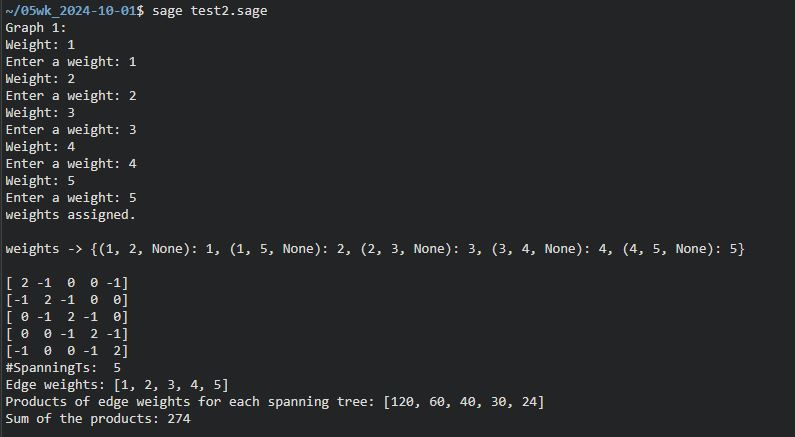
\includegraphics[width=4.2in]{f2.11.jpg}
    \caption{\label{Patch} Same Results for Two Distinctly Distributed C5s}
  \end{center}
	\end{figure}
  
% SUBSECTION 2.2
\subsection{Proof}

Let the two weighted $n$-cycles be denoted as $C_{1}$ and $C_{2}$. The Edges of $C_{1}$ can be represented as $E_{1}=\{e_{1},e_{2},\ldots,e_{n}\}$ and the edges of $C_{2}$ as $E_{2}=\{f_{1},f_{2},\ldots,f_{n}\}$. The weights assigned to the edges of both $C_{1}$ and $C_{2}$ are derived from the same set $W=\{w_{1},w_{2}\ldots,w_{n}\}$ and are assigned randomly; $i.e.,$ for some weight $w_{n}=e_{a}$ and $w_{n}=f_{b}$ where $a,b \le n$. We will define a mapping $m:E_{1}\rightarrow E_{2}$ such that $m(e_{i})=f_{i}$ for $i=1,2,\ldots,n$. To demonstrate that this mapping is a bjection, we must show that it is both injective and surjective. To establish injectivity, suppose there exist indices $i$ and $j$ such that $m(e_{i})=m(e_{j})$. This implies that $f_{i}=f_{j}$. Since the edges $f_{i}$ and $f_{j}$ correspond to distinct connections in the cycle $C_{2}$, we must have $i=j$. Therefore, the mapping $m$ is injective. Next, to show surjectivity, consider any edge $f_{k}\in E_{2}$. There exists an edge $e_{k}\in E_{1}$ such that $m(e_{k})=f_{k}$. This mapping ensures that every edge in $E_{2}$ is accounted for by at least one edge in $E_{1}$, thus satisfying the surjectivity condition. Having established that $m$ is both injective and surjective, we conclude that $m$ is a bijection. This one-to-one correspondence between the edges of $C_{1}$ and $C_{2}$ is independent of the order in which the weights are assigned to the edges. onsequently, since the edges are matched in a bijective manner, the sum of the products of the weights associated with spanning trees of $C_{1}$ and $C_{2}$ remains invariant under the assignments of weights. Thus, the total graph values for both cycles are equal: $$TGV(C_{1})=TGV(C_{2}).$$
$\blacksquare$\\

% SECTION 3
\section{Divided Cycles} \label{DC}
We found that divided cycles behaved rather predictibly since they were essentially cycles with an extra edge. The extra edge seemed to contribute insignificantly to the total overall graph value because it simply wasn't included in many spanning trees. With that being said, we noticed that while assigning the lowest weight to the dividing edge did indirectly contribute to the total graph value, that alone is not enough to determine the max value for any given divided cycle. Other factors, such as the distribution of weights along the cycle edges, played a significant role in determining the total graph value. Specifically, configurations that balanced the weights across the cycle edges while minimizing the impact of the dividing edge on critical spanning tree combinations tended to yield higher graph values. This suggests that the interplay between the edge weights and the structural redundancy of spanning trees in divided cycles must be carefully considered to optimize the total graph value, rather than relying solely on minimizing the weight of the dividing edge.

% SUBSECTION 3.1
\subsection{Code}

% FIGURE 3
	\begin{figure}[h!]  
    \begin{center}
    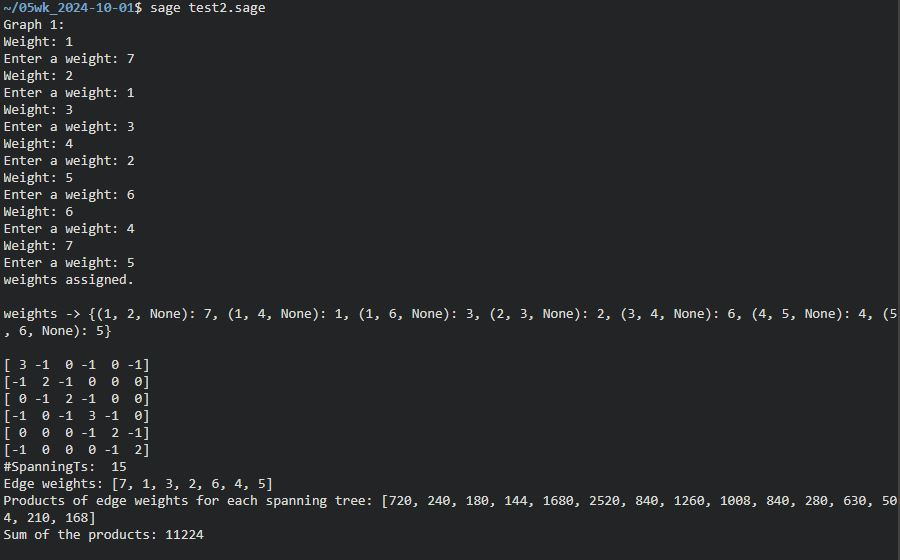
\includegraphics[width=5in]{f3.1.jpg}
    \caption{\label{Marble} The Maximum value for a C6 + 1.}
    \end{center}
	\end{figure}

% FIGURE 4
\begin{figure}[hbt!]  
    \begin{center}
    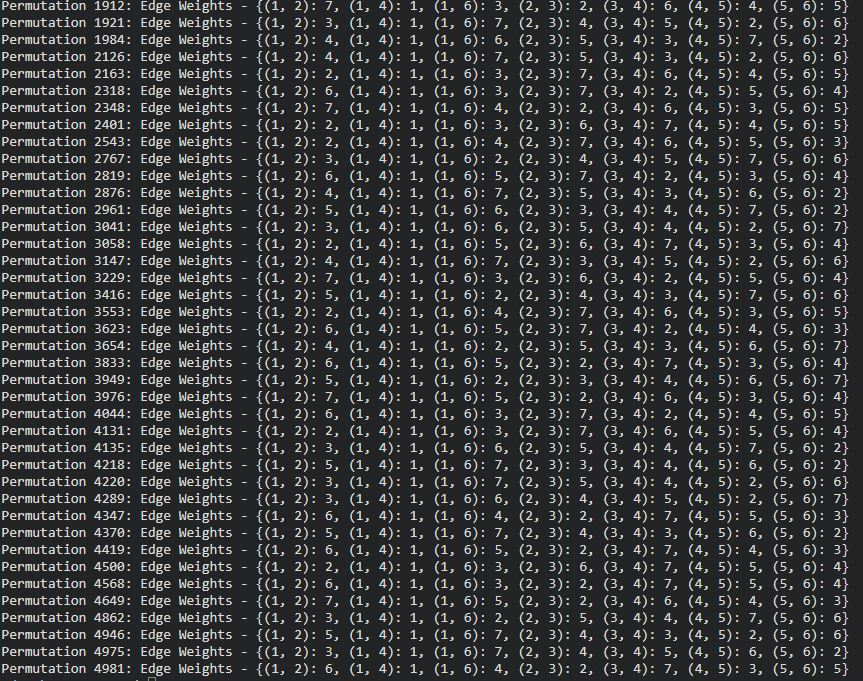
\includegraphics[width=5in]{f3.11.jpg}
    \caption{\label{Marble2} Many C6 + 1 permutations with same max value.}
    \end{center}
	\end{figure}
\newpage
% SUBSECTION 3.2
\subsection{Proof}

Let \( G = C_n + e \) be a graph formed by adding an extra edge \( e \) to an \( n \)-cycle \( C_n \). This additional edge \( e \) connects two non-adjacent vertices in \( C_n \), thereby creating a "divided cycle." Assign weights \( w_1, w_2, \ldots, w_n \) to the edges of \( C_n \) and a weight \( w_{e} \) to the additional edge \( e \). Our goal is to show that the maximum graph value \( V(G) \), which is the sum of the products of the edge weights across all spanning trees of \( G \), is achieved when the smallest weight is assigned to \( e \), with the remaining weights distributed among the edges of \( C_n \).

The graph value \( V(G) \) is defined as
\[
V(G) = \sum_{T \in \mathcal{T}(G)} \prod_{e \in T} w(e),
\]
where \( \mathcal{T}(G) \) denotes the set of all spanning trees in \( G \) and \( w(e) \) represents the weight of edge \( e \).

To calculate \( V(G) \), we consider two types of spanning trees in \( G \): those that include the extra edge \( e \) and those that exclude it. If a spanning tree includes \( e \), it will consist of \( e \) and \( n - 1 \) additional edges chosen from \( C_n \) to span all vertices. If a spanning tree excludes \( e \), it must be formed entirely from the edges in \( C_n \), which results in a spanning tree that is equivalent to a spanning tree of \( C_n \) itself.

We first calculate the number of spanning trees in each case. For the cycle \( C_n \), there are exactly \( n \) spanning trees, as each spanning tree of a cycle graph is formed by removing one of the \( n \) edges in \( C_n \). In \( G \), we have two types of spanning trees: those that include \( e \), of which there are \( n - 1 \), and those that exclude \( e \), of which there are \( n \). Therefore, \( G \) has \( n \) spanning trees that exclude \( e \) and \( n - 1 \) spanning trees that include \( e \). Consequently, spanning trees that exclude \( e \) form the majority of spanning trees in \( G \).

Next, we analyze the effect of weight assignment on the graph value \( V(G) \). Consider the configuration where the smallest weight \( w_{\min} \) is assigned to \( e \), while the remaining, larger weights \( w_1, w_2, \ldots, w_n \) are assigned to the edges of \( C_n \). We now evaluate the contributions to \( V(G) \) from the two cases of spanning trees under this weight assignment.

For spanning trees that include \( e \), each tree’s contribution to the graph value will contain the term \( w_{\min} \) due to the inclusion of \( e \), resulting in a product of the form \( w_{\min} \prod_{i=1}^{n-2} w(e_i) \), where the product is taken over the \( n - 2 \) edges chosen from the \( n-1 \) edges of \( C_n \). Let \( \mathcal{T}_1 \) denote the set of spanning trees in \( G \) that include \( e \). The total contribution from these spanning trees is
\[
V_1 = w_{\min} \sum_{T \in \mathcal{T}_1} \prod_{e \in T \setminus \{e\}} w(e).
\]

Now, consider the effect of assigning \( w_{\min} \) to an edge \( f \) in \( C_n \) instead of \( e \). If \( f \) has weight \( w_{\min} \), the contributions from spanning trees that exclude \( e \) will involve products containing \( w_{\min} \), while those that include \( e \) will no longer gain the benefit of a small weight on \( e \). We compare this to the case where \( w_{\min} \) is assigned to \( e \):\\

\textbf{Case 1: Assign \( w_{\min} \) to \( e \)}

The contribution \( V_1 \) from spanning trees including \( e \) is minimized due to the small \( w_{\min} \), while \( V_2 \), the contribution from spanning trees excluding \( e \), is maximized because the larger weights are concentrated on the edges of \( C_n \). This configuration ensures that the graph value \( V(G) = V_1 + V_2 \) is as large as possible.\\

\textbf{Case 2: Assign \( w_{\min} \) to \( f \in C_n \)}

Now, spanning trees that exclude \( e \) will include \( f \) with weight \( w_{\min} \). The contribution \( V_2 \) is reduced because every spanning tree in \( \mathcal{T}_2 \) will contain the smaller \( w_{\min} \) in its product. Additionally, the contribution \( V_1 \) from spanning trees including \( e \) is not minimized as effectively, because \( e \) now has a larger weight. This results in a smaller total graph value \( V(G) \).\\

To see this effect explicitly, note that \( V_2 \) in Case 2 is proportional to
\[
w_{\min} \cdot \sum_{T \in \mathcal{T}_2'} \prod_{e \in T \setminus \{f\}} w(e),
\]
where \( \mathcal{T}_2' \) is the set of spanning trees in \( C_n \) that include \( f \). Since \( \mathcal{T}_2' \) contains \( n-1 \) trees, the factor of \( w_{\min} \) uniformly reduces the contribution from all these spanning trees. By contrast, in Case 1, \( V_2 \) does not include \( w_{\min} \), allowing the larger weights to dominate the product.

Thus, assigning \( w_{\min} \) to any edge \( f \in C_n \) reduces \( V(G) \) compared to assigning it to \( e \). This proves that placing the smallest weight \( w_{\min} \) on the extra edge \( e \) maximizes the graph value \( V(G) \).

$\blacksquare$\\

% PART 2
\part{Comments on Complete Graphs and others} \label{Kn}

We were unable to find a general solution for complete graphs but we were able to find some interesting results that are still worth mentioning.

% SECTION 4
\section{$K_{4}$ Results}

For $K_{4}$ we were able to determine total graph value and all its permutations via its Hamiltonian cycles. Due to its symmetry we believe that all of these max permutations are isomorphic to each other but did not prove this rigorously enough to arrive at a satisfactory answer.

% FIGURE 5
\begin{figure}[hbt!]  
    \begin{center}
    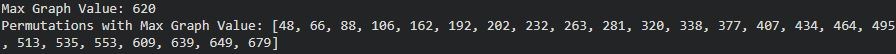
\includegraphics[width=6in]{f4.1.jpg}
    \caption{\label{last} All Permutations of K4 with Max Value.}
    \end{center}
	\end{figure}
  

% SECTION 5
\section{$K_{5}$ Limitations}

For $K_{5}$ we ran into hardware limitations as the processing load became too massive to fully compile in a reasonable amount of time. While we were unable to determine the maximum graph value for $K_{5}$, we were able to work around this slightly by using a pseudo-random permutation generator and fixed weights to lessen the burden on the processor.

	\newpage \listoffigures 
\end{document}